\section{Pregunta N$^{\circ}$10\qquad Carlos Daniel Malvaceda Canales}

\begin{frame}
	\begin{enumerate}\setcounter{enumi}{9}
		\item

		      Determinar gráficamente el número de raíces reales de la
		      ecuación no lineal
		      \begin{math}
			      x\ln\left(x\right)=
			      1
		      \end{math}
		      y resuelve usando los métodos de la bisección, la regla
		      falsa y la regla falsa modificada para $\epsilon=10^{-5}$.
	\end{enumerate}

	\begin{solution}

		\begin{figure}
			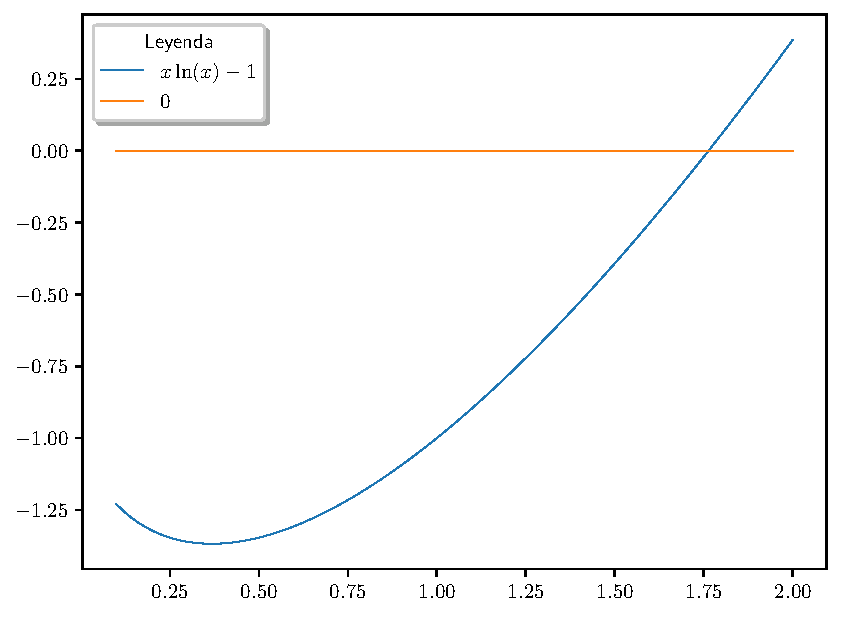
\includegraphics[width=0.5\paperwidth]{p10.pdf}
			% \caption{.}
		\end{figure}

	\end{solution}
\end{frame}